\section{Hypothèses et formules}
\label{sec:hypotheses}
\subsection{Notation}
L'article ne montre pas explicitement la manière d'attribuer une note à une performance dont l'agent gagne une certaine utilité. Toutefois les intervalles de ces deux valeurs sont précisés : $UG \in [-10;10]$ et $v \in [-1;1]$. Nous avons opté pour la manière la plus simple de noter, $v = UG/10$ mais il est possible de biaiser cette notation (selon des agents dont le comportement serait différent par exemple). Cette alternative peut être intéressante si l'application du modèle le requiert. 

Enfin, étant donné que les performances sont tirées selon une distribution normale autour des moyennes, il se peut qu'elles dépassent [-10;10]. Dans ces cas, le programme remet les valeurs dans l'intervalle.

\subsection{Rayon d'opération}
L'article ne décrit pas la manière de choisir le rayon d'opération. Nous avons donc posé deux intervalles dans lesquelles les agents tirent une valeur aléatoirement pour définir leur rayon d'opération. Pour plus de réalisme, nous avons décidé d'attribuer, en général, un rayon plus grand pour les fournisseurs que pour les consommateurs. En effet, l'article compare le rayon d'opération d'un fournisseur à la distance entre deux grandes régions du monde (pays, continent...) et celui d'un consommateur à un voisinage proche. Cette même logique a été appliqué à notre modèle.
On a donc $C_{R_o} \in [0.1;0.4]$ et $P_{R_o} \in [0.5;1]$


\subsection{Régression de l'utilité en fonction de la distance}
Lorsqu'un agent consommateur ne se situe pas dans le rayon d'opération d'un fournisseur, la performance qui résulte de l'interaction en sera affecté. Par conséquent l'utilité sera dégradée (linéairement). En l'absence de données, nous avons dû déterminé le facteur de régression pour cette fonction. Le facteur :\[ \alpha = \frac{1}{c*D_{MAX}} \]. 

\emph{c} : ce coefficient permet de mesurer l'impact qu'aura la distance sur l'UG. Plus c sera grand moins une performance sera modifiée et plus c sera petit plus la distance qui sépare un consommateur (hors de portée) d'un fournisseur impactera l'UG. Dans notre cadre, nous le fixons à 100.

$D_{MAX}$ : la distance maximum qui peut séparer deux agents situé sur une sphère de rayon R. Nous considérons qu'il s'agit de la moitié de la circonférence du grand cercle c'est-à-dire \[ D_{MAX} = \pi * R \].

Ainsi, si l'utilité sera affecté de la manière suivante  \[ UG = UG - ( |UG|*(d-r_o)*\alpha\]. où $(d-r_o)$ représente la distance qui sépare le consommateur de rayon d'opération du fournisseur.

Cette régression devra être prise en compte lorsqu'une information concernant un fournisseur vient d'une tierce personne. En effet quand le consommateur \texttt{a} demande au consommateur \texttt{c} la note qu'il a mis pour le fournisseur {b}, il faut prendre en compte, en plus de la différence de temps $\delta$t(comme décrit dans l'article), la différence de distance. Nous cherchons donc à estimer l'\texttt{UG1} que l'agent \texttt{a1} tirera de l'interaction en connaissant l'\texttt{UG2} que l'agent \texttt{a2} a eu de cette façon : \[ UG1 = UG2 + \delta UG\].
avec
\[ \delta UG = \alpha*(d_2-d_1) \]
Étant donné que l'écart $\delta$UG ajouté dépend de la différence de distance entre a1 et a2, dans le cas d'une interaction directe (a1=a2), on aura bien $\delta$UG = 0.


\subsection{Calcul de distance}
Pour déterminer la distance qui sépare deux agents, nous avons décidé d'utiliser la distance du grand cercle plutôt qu'une distance euclidienne car plus représentative du monde réel (sphérique).

\begin{figure}[h!]
\centering
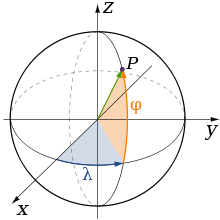
\includegraphics[scale=0.5]{images/great-circle-distance-img.png}
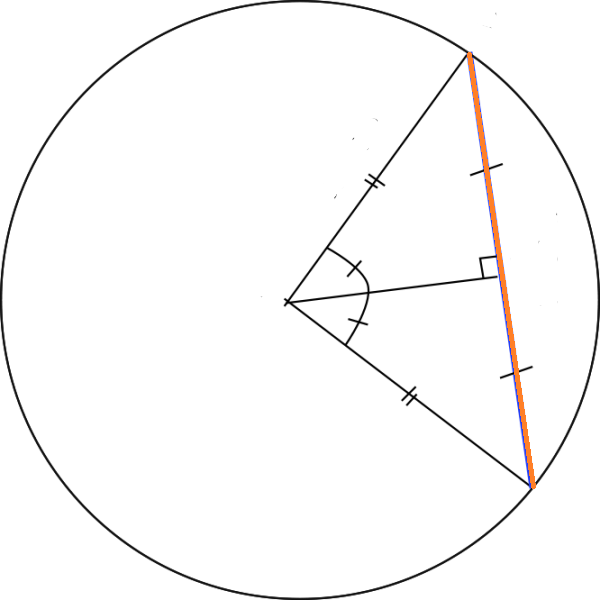
\includegraphics[scale=0.2]{images/distance-euclidienne.png}
\caption{Distance du grand cercle - Distance euclidienne}
\label{fig:Distance du grand cercle}
\end{figure}

Pour ce faire, nous avons eu besoin de convertir les coordonnées (cartésiennes par défaut) selon les formules suivantes \cite{conversion} : 

Cartésiennes -> Polaires
\[
   r = \sqrt{x^2 +y^2 + z^2} 
  \].
   \[
  \theta = \arccos\frac{z}{r}
    \].
     \[
  \phi = \arctan\frac{y}{x}
\].

Polaires -> Cartésiennes
\[
   x = r\sin{\theta}\cos{\phi}
  \].   
   \[
   y = r \sin{\theta}\sin{\phi}
   \]. 
    \[
   z = r\cos{\theta}
\].

La distance sera ensuite déterminée ainsi \cite{distance} :

\[ D = R\arcsin{\frac{d\sqrt{4R^2-d^2}}{2R^2}} \].
avec $ d^2 = (x_1-x_2)^2 + (y_1-y_2)^2 + (z_1-z_2)^2 $

\subsection{Température \cite{Dilemme}}
\label{sec:temperature}
La température est un facteur apparaissant dans le dilemme de Boltzmann mais dont la valeur dépend totalement de l'application.
Après de multiples changements et tests, elle a finalement été initialisé à 500 (le nombre d'interactions pour une simulation) et est décrementée à chaque tour.
